\section{Результаты работы и ускорение}
Чтобы проверить эффективность работы алгоритма параллельной записи, описанного в \ref{sec1}, проведено сравнение с алгоритмом стандартной печати: \vspace{12pt}
\begin{spacing}{0.75}
\texttt{
\begin{tabular}{ll}
 $\quad$ & for (int i = 0; i < n;)\\
 $\quad$ & $\,\,$ \{ \\
 $\quad$ & $\,\,\quad$ for (int j = 0; j < m; j++, i++)\\
 $\quad$ & $\,\,\quad\quad$ fprintf (f, '' \%.16f'', a[i]);\\
 $\quad$ & $\,\,\quad$ fprintf (f, ''$\mathtt{\backslash n}$''); \\
 $\quad$ & $\,\,$ \} \\
\end{tabular}}\\
\end{spacing}
Здесь $n$ -- размер массива, а $m$ -- количество чисел, записываемых в одну строку.
Стандартная печать будет записывать числа с 16 знаками после запятой.

Для всех дальнейших тестов было сделано следующее.
Оба выходных файла, полученные работой параллельного алгоритма и стандартного, считывались вновь. 
Затем вычислялась разница между считанным числами.
Во всех запусках погрешность не превышала машинной точности, что говорит о точности работы реализованного алгоритма.

\subsection{Тест 1. Массив случайных чисел} \label{t1}
Оба алгоритма запускались на одних и тех же массивах вещественных чисел, сгенерированных случайным образом. 
Этот тест полезен тем, что в реальных моделях данные могут задаваться каким-либо распределением (например, нормальным), где все числа являются вещественными и различными.

Описанный в Разделе \ref{sec1} алгоритм параллельной записи запускался с разным числом потоков.

Время работы в секундах для обоих алгоритмов приведено в Таблице 1.
Под числом потоков понимается число потоков-обработчиков. 
Таким образом реально задействовано на два потока больше, так как помимо обработчиков есть еще управляющий поток и печатающий.
\begin{center}
\begin{tabular}{||c|c|c|c|c|c||}
\hline
\hline
Размер & \multicolumn{4}{c|}{Число потоков} & Стандартная\\
\hhline{~|-|-|-|-|~|}
массива & 16 & 12 & 4 & 1 & печать \\
\hline
\hline
& 0.609 & 0.550 & 0.880 & 3.196 & 4.256 \\
\hhline{~|-|-|-|-|-|}
$10^7$ & 0.567 & 0.500 & 0.841 & 3.239 & 4.176 \\
\hhline{~|-|-|-|-|-|}
& 0.506 &0.473 & 0.802 & 3.052 & 4.188 \\
\hline
& 2.420 & 2.528 & 4.044 & 15.377 & 22.476 \\
\hhline{~|-|-|-|-|-|}
$5 \cdot 10^7$  & 2.522 & 2.446 & 4.273 & 16.309 & 21.116\\
\hhline{~|-|-|-|-|-|}
& 2.587 & 2.339 & 4.179 & 15.327 & 20.893 \\
\hline
& 5.025 & 4.665 & 8.276 & 32.461 & 41.712 \\
\hhline{~|-|-|-|-|-|}
$10^8$  & 4.787 & 4.630 & 7.970 & 30.571 & 41.785 \\
\hhline{~|-|-|-|-|-|}
& 4.844 & 4.544 & 8.078 & 30.757 & 41.961 \\
\hline
& 21.199 & 20.074 & 37.515 & 148.548 & 201.941 \\
\hhline{~|-|-|-|-|-|}
$5 \cdot 10^8$  & 21.312 & 20.297 & 37.627 & 148.829 & 202.333 \\
\hhline{~|-|-|-|-|-|}
 & 21.231 & 20.171 & 37.686 & 149.217 & 201.692 \\
\hline
\hline
\end{tabular}\\ \vspace{10pt}
\small{Таблица 1.}
\end{center}
Заметим, что время работы на шестнадцати потоках несколько больше, чем на двенадцати. 
Это обусловлено тем, что алгоритм запускался на машине с двенадцатью ядрами.
Таким образом в первом случае число потоков превосходило число ядер, и имели место накладные расходы.

Также стоит заметить, что отношение времени работы при увеличении количства потоков заметно уменьшается, и при увеличении размеров массива стремится к обратному отношению числа потоков.
Тот факт, что эти отношения не строго равны объясняется сразу несколькими факторами.
Во-первых, часть времени, хоть и небольшую при таких данных, занимала запись на диск.
Во-вторых, не все потоки могли быть все время задействованными.
Некоторые потоки могли обращаться к пустой очереди и тем самым тратить время на ожидание.

Размер полученного файла, а также среднее ускорение работы алгоритма по сравнению со стандартной печатью приведены в следующей Таблице 2:
\begin{center}
\begin{tabular}{||c|c|c|c|c|c||}
\hline
\hline
Размер & \multicolumn{4}{c|}{Число потоков} & Размер\\
\hhline{~|-|-|-|-|~|}
массива & 16 & 12 & 4 & 1 & файла \\
\hline
$10^7$ & 7.50 & 8.20 & 5.00 & 1.33 & 245 MB \\
\hline
$5 \cdot 10^7$ & 8.57 & 8.80 & 5.16 & 1.37 & 1.2 GB \\
\hline
$10^8$ & 10.61 & 11.23 & 6.39 & 1.66 & 2.4 GB\\
\hline
$5 \cdot 10^8$ & 9.51 & 10.01 & 5.37 & 1.36 & 12 GB \\
\hline
\hline
\end{tabular}
\\\vspace{10pt}
\small{Таблица 2.}
\end{center}

Заметим, что при увеличении массива до определенного размера, ускорение возрастает, а затем спадает.
Первое объясняется тем, что с увеличением объема данных, потоки простаивают меньше.
Второй факт будет рассмторен подробнее в пункте \ref{subsec2:3}.

\subsection{Тест 2. Повторяющиеся числа}
Сгенереруем массив чисел из 0 и 1.
В этом случае все последовательности одинаковых подряд идущих чисел будут сворачиваться в короткую строку вида \texttt{n*x}.

Также с помощью этого теста во-первых можно проверить работу с целыми числами, а во-вторых убедиться в том, что \textsf{Grisu2} отбрасывает ненужные нули.

Были сделаны замеры времени аналогично предыдущему тесту.
Время работы в секундах приведено в Таблице 3:
\begin{center}
\begin{tabular}{||c|c|c|c|c|c||}
\hline
\hline
Размер & \multicolumn{4}{c|}{Число потоков} & Стандартная\\
\hhline{~|-|-|-|-|~|}
массива & 16 & 12 & 4 & 1 & печать \\
\hline
\hline
& 0.318 & 0.249 & 0.188 & 0.652 & 3.645 \\
\hhline{~|-|-|-|-|-|}
$10^7$ & 0.334 & 0.256 & 0.190 & 0.629 & 3.622 \\
\hhline{~|-|-|-|-|-|}
& 0.307 & 0.251 & 0.192 & 0.661 & 3.620 \\
\hline
& 1.657 & 1.274 & 0.884 & 3.183 & 18.412 \\
\hhline{~|-|-|-|-|-|}
$5 \cdot 10^7$ & 1.505 & 1.247 & 0.891 & 3.167 & 18.306 \\
\hhline{~|-|-|-|-|-|}
& 1.522 & 1.262 & 0.894 & 3.175 & 18.261 \\
\hline
& 3.105 & 2.441 & 1.726 & 6.306 & 36.194 \\
\hhline{~|-|-|-|-|-|}
$10^8$ & 2.983 & 2.453 & 1.820 & 6.329 & 36.388 \\
\hhline{~|-|-|-|-|-|}
& 3.246 & 2.505 & 1.759 & 6.339 &  36.419 \\
\hline
& 16.194 & 12.575 & 8.681 & 31.505 & 181.221 \\
\hhline{~|-|-|-|-|-|}
$5 \cdot 10^8$ & 16.414 & 12.564 & 8.787 & 31.291 & 181.406 \\
\hhline{~|-|-|-|-|-|}
& 15.815 & 12.555  & 8.764 & 31.690 & 182.524 \\
\hline
\hline
\end{tabular}
\\\vspace{10pt}
\small{Таблица 3.}
\end{center}
Среднее ускорение приведено в Таблице 4.
Также приведен размер файла ''со звездами'', полученным быстрым алгоритмом, и размер файла ''без звезд'', полученного алгоритмом стандартной печати.

\begin{center}
\begin{tabular}{||c|c|c|c|c|c||}
\hline
\hline
Размер & \multicolumn{4}{c|}{Число потоков} & Размер\\
\hhline{~|-|-|-|-|~|}
массива & 16 & 12 & 4 & 1 & файла \\
\hline
$10^7$  & 11.35 & 14.40 & 19.10 & 5.61 & 24 MB / 187 MB \\
\hline
$5 \cdot 10^7$ &11.74 & 14.53 & 20.60 & 5.77 & 123 MB / 936 MB\\
\hline
$10^8$ &11.68 & 14.73 & 20.55 & 5.74 & 245 MB / 1.8 GB \\
\hline
$5 \cdot 10^8$ &11.26 & 14.46 & 20.78 & 5.77 & 1.2 GB / 9.4 GB\\
\hline
\hline
\end{tabular}
\\\vspace{10pt}
\small{Таблица 4.}
\end{center}

Если сравнить эту таблицу с аналогичной в предыдущем пункте, то можно заметить, что ускорения возросли.
Это произошло засчет того, что благодаря записи со звездами, заметно уменьшился и размер выходного файла, а как следствие уменьшилось и время работы.

\subsection{Тест 3. Огромные массивы} \label{subsec2:3}
Здесь, как и в первом случае, числа будут генерироваться случайным образом.
Сравнивать будем стандартную печать и алгоритм, запущенный на 12 (+2) потоках.

Помимо обычного запуска, проведем и запуск с записью не на диск, а в разделяемую память \textit{shared-memory}.
Как известно, разделяемая память является самым быстром средством обмена данными между проессами.

Ранее говорилось, что скорость диска влияет на печать, но не всегда сильно.
Засчет сравнения записи на диск и в \textit{shared-memory} можно оценить, это влияние.

Далее на Рисунке \ref{grap} приведена зависимость времени работы от размера массива.
\begin{figure}[H]
\center{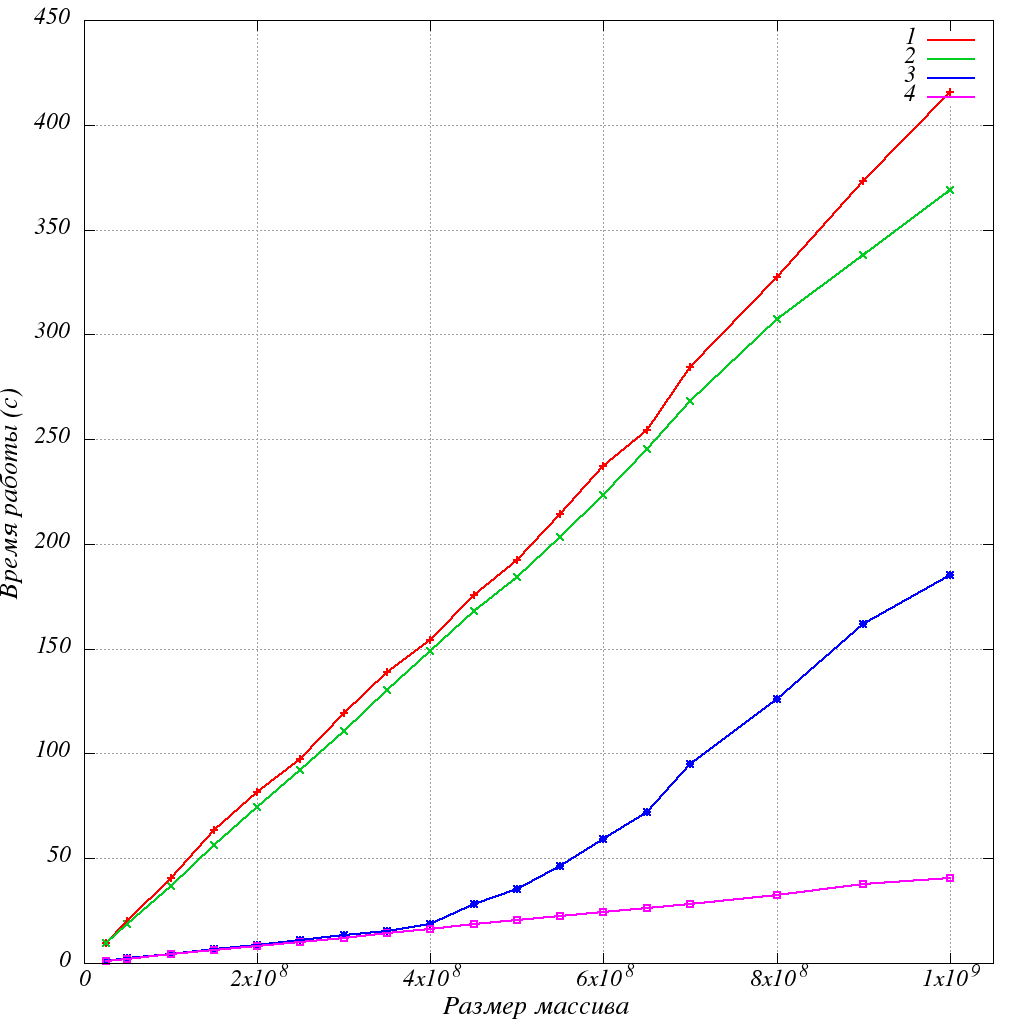
\includegraphics[width=1\linewidth]{./pics/graphics.png}}
\caption{
1 -- стандартная печать с записью на диск;
2 -- стандартная печать с записью в разделяемую память;
3 -- алгоритм параллельной печати с записью на диск;
4 -- алгоритм параллельной печати с записью в разделяемую память.} \label{grap}
\end{figure}

Сначала хочется заметить, что стандартная печать не сильно замедляется при записи в диск. 
Все время скорость работы диска была порядка 40--50 Mb/s.
Диск фактически не оказывает никакого существенного влияния на работу.

Из графиков также видно, что при записи в \textit{shared-memory} отношение времени работы стандартного алгоритма и ускоренного постоянно, так как оба графика -- прямые.
Это значит, что ускорение одинакого на всех данных.

Однако, такого нельзя сказать в случае записи на диск.
На графике в точке $4 \cdot 10^8$ (9.6 GB) происходит излом: начинает ощущаться влияние диска. Именно это мы и наблюдали в Тесте 1 -- ускорение немного упало при $5 \cdot 10^8$.
С этого момента печать начинает упираться в диск.
При запуске тестов было замечено, что скорость записи на диск временами достигает 800-900 Mb/s.
Из-за слишком больших файлов (так файл при размере массива $10^9$ достигает 24 GB) создается очередь из буфферов на печать.
Потоки-обработчики обрабатывают буфферы быстрее, чем производится сама печать.
Разница между третьим и четвертым графиком -- накладные расходы на работу диска.

\subsection{Тестирование на реальных моделях}
?????

\vspace{10pt}

\begin{tabular}{||l||c|c|c||}
\hline
\hline
& Время работы & Время работы & Ускорение \\
\hline
\hline
COORD & 0.028 & 0.003 & 9.33 \\
\hline
ZCORN & 0.135 & 0.013 & 10.38 \\
\hline
COORD & 0.132 &  0.010 & 13.2 \\
\hline
ZCORN & 12.819 & 0.982 & 13.05 \\
\hline
\hline
\end{tabular}

